\documentclass[tikz,border=5pt]{standalone}
\usepackage{amsmath,amssymb}
\usepackage{tikz}
\usetikzlibrary{calc,arrows.meta}
\begin{document}
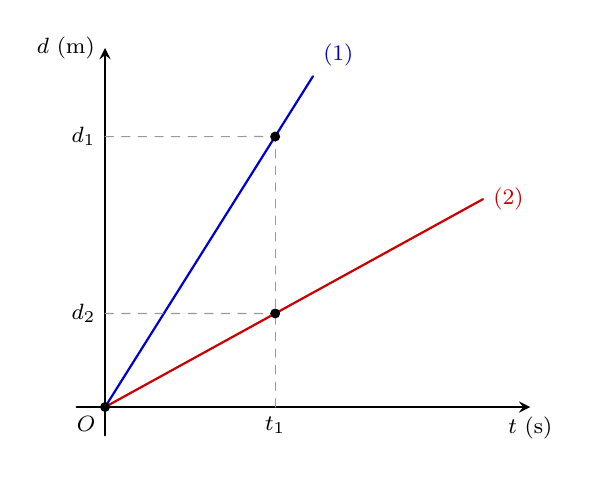
\begin{tikzpicture}[>=stealth, line join=round, line cap=round, font=\footnotesize, scale=1.2]
    % Trục tọa độ
    \draw[->, thick] (-0.3, 0) -- (4.5, 0) node[below] {$t\text{ (s)}$};
    \draw[->, thick] (0, -0.3) -- (0, 3.8) node[left] {$d\text{ (m)}$};
    \node[below left] at (0, 0) {$O$};
    
    % Hai đường đồ thị d - t
    \draw[thick, blue!80!black] (0, 0) -- (2.2, 3.5) node[above right] {$(1)$};
    \draw[thick, red!80!black] (0, 0) -- (4.0, 2.2) node[right] {$(2)$};
    
    % Đường dóng tại thời điểm t1
    \def\tval{1.8}
    \coordinate (T1) at (\tval, 0);
    \coordinate (P2) at (\tval, {0.55*\tval});
    \coordinate (P1) at (\tval, {1.59*\tval});
    
    \draw[dashed, gray!80] (T1) -- (P1);
    \draw[dashed, gray!80] (0, {0.55*\tval}) node[left, black] {$d_2$} -- (P2);
    \draw[dashed, gray!80] (0, {1.59*\tval}) node[left, black] {$d_1$} -- (P1);
    
    \node[below] at (T1) {$t_1$};
    
    \fill[black] (P1) circle (1.5pt);
    \fill[black] (P2) circle (1.5pt);
    \fill[black] (0,0) circle (1.5pt);
\end{tikzpicture}
\end{document}
